\documentclass{beamer}

\usetheme{default}
%\usecolortheme{seahorse}
%\usecolortheme{beaver}
%\usetheme{Warsaw}
\usecolortheme{crane}
%\usetheme{Warsaw}
%\setbeamercolor{structure}{fg=cyan!90!black}
\setbeamercolor{titlelike}{parent=whale,fg=yellow!85!white,bg=violet!55!black} %bg=yellow!85!orange}
% \definecolor{craneorange}{rgb}{0.68,1,1}
%\definecolor{craneblue}{gray}{0.85}


%\documentclass[compress,greek]{beamer}
%\mode<presentation>
%{
%\usetheme{default}\usecolortheme{beaver}%\useoutertheme{default}
%\usetheme{PaloAlto}
% \usetheme{Warsaw} %<-- Well known blue theme
% \usetheme{Berlin}
%\usecolortheme{seahorse}
%\usecolortheme{rose}
%\usetheme{Berkeley}
%\usetheme{boxes}
%\usetheme{Antibes}
% \usetheme{Bergen}
%\usetheme{CambridgeUS} %<-- Simpler themes I like
% \usetheme{Copenhagen}
% \usetheme{Darmstadt}
%\usetheme{Dresden}
% \usetheme{Frankfurt}
%\usetheme{Goettingen} %<-- Simpler themes I like
% \usetheme{Hannover}
%\usetheme{Ilmenau}
% \usetheme{JuanLesPins}
% \usetheme{Luebeck}
%\usetheme{Madrid}
%\usetheme{Malmoe}
% \usetheme{Marburg} %<-- Simpler themes I like
%\usetheme{Montpellier}
% \usetheme{Pittsburgh}
% \usetheme{Rochester}
% \usetheme{Singapore} %<-- Simpler themes I like
%\usetheme{Szeged}
%\usetheme{Boadilla}
%\usetheme{AnnArbor}

%%% remove beamer's navigation bar!! %%%%%%
% \setbeamertemplate{navigation symbols}{} %% 
%%%%%%%%%%%%%%%%%%%%%%%%%%%%%%%%%%%%%%%%%%%

%%%% Comment to completely cover next transparencies %%
%\setbeamercovered{transparent} %%%%%%%%%%%%%%%%%%%%%%%%
%%%%%%%%%%%%%%%%%%%%%%%%%%%%%%%%%%%%%%%%%%%%%%%%%%%%%%%
%}

%\usepackage{babel}
%\usepackage[iso-8859-7]{inputenc}


%%% FONT SELECTION %%%%%%%%%%%%%%%%%%%%%%
%%% we choose a sans font %%%%%%%%%%%%%%%
%\usepackage{kmath,kerkis} %%%%%%%%%%%%%%

%\usepackage[default]{gfsneohellenic} %%%%

%%%%%%%%%%%%%%%%%%%%%%%%%%%%%%%%%%%%%%%%%

\usepackage{color}
\usepackage{amsmath}
%\usepackage{amssymb}
\usepackage{hyperref}
\usepackage{amsfonts,amssymb,wasysym}
\usepackage[accumulated]{beamerseminar}
\usepackage{beamertexpower}

\usepackage{xcolor}
\definecolor{mediumseagreen}{rgb}{0.24,0.7,0.44}
\definecolor{seagreen}{rgb}{0.18,0.55,0.34}

\usepackage[T1]{fontenc}

\usepackage{booktabs}
\usepackage{lmodern}

\usepackage{tikz}
\usepackage{pgf}
\usetikzlibrary{arrows,shapes,trees,topaths,petri,shapes.arrows}
\usetikzlibrary{automata,positioning}
\usetikzlibrary[automata]
\usepackage{verbatim}

\usepackage{listings}

\lstset{
  literate={ö}{{\"o}}1
           {ä}{{\"a}}1
           {ü}{{\"u}}1
}

\usepackage{subfigure}

\usepackage{soul}

\makeatletter
\let\HL\hl
\renewcommand\hl{%
  \let\set@color\beamerorig@set@color
  \let\reset@color\beamerorig@reset@color
  \HL}
\makeatother
  
\DeclareSymbolFont{extraup}{U}{zavm}{m}{n}
\DeclareMathSymbol{\varheart}{\mathalpha}{extraup}{86}
\DeclareMathSymbol{\vardiamond}{\mathalpha}{extraup}{87}

\DeclareMathOperator{\degr}{deg}
\DeclareMathOperator{\rec}{Recip}
\DeclareMathOperator{\cog}{Co--Giv}
\DeclareMathOperator{\cor}{Co--Rec}

\DeclareMathOperator{\tr}{tr}
\DeclareMathOperator{\med}{med}
\DeclareMathOperator{\Aut}{Aut}

\DeclareMathOperator{\pre}{pre}
\DeclareMathOperator{\post}{post}

\makeatletter
% %%%%%%%%%%%%%%%%%%%%%%%%%%%%%% Textclass specific LaTeX commands.
  % this default might be overridden by plain title style
  \newcommand\makebeamertitle{\frame{\maketitle}}%
  \AtBeginDocument{
    \let\origtableofcontents=\tableofcontents
    \def\tableofcontents{\@ifnextchar[{\origtableofcontents}{\gobbletableofcontents}}
    \def\gobbletableofcontents#1{\origtableofcontents}
  }
  \makeatletter
  \long\def\myframe#1{\@myframe#1\@myframestop}%
  \def\@myframe{\@ifnextchar<{\@@myframe}{\@@myframe<*>}}%
  \def\@@myframe<#1>{\@ifnextchar[{\@@@myframe<#1>}{\@@@myframe<#1>[]}}
  \def\@@@myframe<#1>[{\@ifnextchar<{\@@@@@myframe<#1>[}{\@@@@myframe<#1>[<*>][}}
  \def\@@@@@myframe<#1>[#2]{\@ifnextchar[{\@@@@myframe<#1>[#2]}{\@@@@myframe<#1>[#2][]}}
  \long\def\@@@@myframe<#1>[#2][#3]#4\@myframestop#5\myframeend{%
    \frame<#1>[#2][#3]{\frametitle{#4}#5}}
  \makeatother
  \newenvironment{topcolumns}{\begin{columns}[t]}{\end{columns}}
  \def\myframeend{} % In case there is a superfluous frame end

%%% remove beamer's navigation bar!! %%%%%%
% \setbeamertemplate{navigation symbols}{} %% 
%%%%%%%%%%%%%%%%%%%%%%%%%%%%%%%%%%%%%%%%%%%

%%%% Comment to completely cover next transparencies %%
\setbeamercovered{transparent} %%%%%%%%%%%%%%%%%%%%%%%%
%%%%%%%%%%%%%%%%%%%%%%%%%%%%%%%%%%%%%%%%%%%%%%%%%%%%%%%

\makeatother

%%%%%%%%%%%%%%%%%%%%%%%%%%%%%%%%%%%%%%%%%%%%%%%%%%%%%%%%%%%%

\newtheorem{prop}{�������}
%\setbeamercolor{block body prop}{fg=white,bg=red}
%\newtheorem{defs}{�������}}

%\newtheorem{theorema}{\translate{�������}}
%\setbeamercolor{block body theorema}{fg=white,bg=red}

%\newdefinition{symbs}{�����������}

\newtheorem{lima}{�����}

\let\OLDtheorem=\theorem
\def\theorem{%
  \setbeamercolor{block title}{fg=white,bg=violet}%
%  \setbeamercolor{block title}{fg=red!75!black,bg=yellow!75!black}%
%  \setbeamercolor{block body}{fg=red,bg=yellow}\OLDtheorem
  \setbeamercolor{block body}{fg=black}\OLDtheorem
}

\let\OLDprop=\prop
\def\prop{%
  \setbeamercolor{block title}{fg=white,bg=olive}%
  \setbeamercolor{block body}{fg=black}\OLDprop
}

\let\OLDCorollary=\Corollary
\def\Corollary{%
  \setbeamercolor{block title}{fg=white,bg=brown}%
  \setbeamercolor{block body}{fg=black}\OLDCorollary
}

\let\OLDlima=\lima
\def\lima{%
  \setbeamercolor{block title}{fg=black,bg=yellow}%
  \setbeamercolor{block body}{fg=black}\OLDlima
}






\begin{document}

\newenvironment{tightcenter}{%
  \setlength\topsep{0pt}
  \setlength\parskip{0pt}
  \begin{center}
}{%
  \end{center}
}

\title[Financial Exchange Networks]{Financial Exchange Networks Among Political Committees in the 2020 Election Cycle}
\author[Lobue\&Boudourides]{{\color{blue}David LoBue\!\! \inst{1} and Moses A. Boudourides\!\! \inst{1,2}}\\[2ex]
{\inst{1} \scriptsize{Master's in Data Science Online Program\\
School of Professional Studies \\ 
Northwestern University\\%[1.3ex]
{\href{mailto:davidlobue2021@u.northwestern.edu}{\texttt{\textcolor{teal}
{davidlobue2021@u.northwestern.edu}}}} and 
{\href{mailto:Moses.Boudourides@northwestern.edu}{\texttt{\textcolor{teal}{Moses.Boudourides@northwestern.edu}}}}\\[1ex]  
}}
{\inst{2} \scriptsize{Professor of Practice\\ 
School of Public Affairs\\
Arizona State University\\%[1.3ex]
\vspace{-1.5 mm}
{\href{mailto:Moses.Boudourides@asu.edu}{\texttt{\textcolor{teal}{Moses.Boudourides@asu.edu}}}}
\vspace{-7 mm}
}} 
 }
%\date{June, 2014}
\date[PolNet] % (optional, should be abbreviation of conference name)
{{\it{Political Networks Conference ({\bf{PolNet 2022}})}}\\[0.2ex]
{\scriptsize{Hosted Virtually by University of Iowa}}\\[0.2ex]
% {\small{Virtual}}\\[0.8ex]
{\small{{\it{American Institutions \& Interest Groups}} Panel}}\\[0.2ex] 
{July 13, Wednesday, 12:30 PM - 2:00 PM,  CT}}

\makebeamertitle


\begin{frame}
\frametitle{Table of Contents}


\begin{description}

\item[$\vardiamond$] {\hyperlink{L1}{\beamergotobutton{\color{yellow}{From Data to Networks}}}} \\[3ex]

%\begin{itemize}
%\item {\hyperlink{L1a}{\beamergotobutton{\color{yellow}{Data Source}}}}
%\item {\hyperlink{L1b}{\beamergotobutton{\color{yellow}{The Directed Graph of Exchanges among Committees}}}}
%\item {\hyperlink{L1c}{\beamergotobutton{\color{yellow}{Political Affiliation of Committees}}}}
%\end{itemize}

\item[$\clubsuit$] {\hyperlink{L2}{\beamergotobutton{\color{yellow}{Dyadic \& Triadic Methods}}}} \\[3ex]

%\begin{itemize}
%\item {\hyperlink{L2a}{\beamergotobutton{\color{yellow}{Dyads \& Triads}}}}
%\item {\hyperlink{L2b}{\beamergotobutton{\color{yellow}{Reciprocating Dyads \& Co--Giving or Co--Receiving Triads}}}}
%\item {\hyperlink{L2c}{\beamergotobutton{\color{yellow}{Closures of Reciprocating Dyads \& Co--Giving or Co--Receiving Triads}}}} %and Citation Graphs
%\item {\hyperlink{L2d}{\beamergotobutton{\color{yellow}{Co--Giving \& Co-Receiving Triads \& Graphs}}}}
%\end{itemize}

\item[$\spadesuit$] {\hyperlink{L3}{\beamergotobutton{\color{yellow}{Graphs of Dyads \& Triads of Committees Labelled in Political Affiliation}}}} \\[3ex]

%\begin{itemize}
%\item {\hyperlink{L3a}{\beamergotobutton{\color{yellow}{The Graph of Aggregated Committees in Political Affiliation}}}}
%\item {\hyperlink{L3b}{\beamergotobutton{\color{yellow}{Graphs of Labelled Reciprocation}}}}
%\item {\hyperlink{L3c}{\beamergotobutton{\color{yellow}{Graphs of Labelled Co--Giving Triads}}}}
%\item {\hyperlink{L3d}{\beamergotobutton{\color{yellow}{Graphs of Labelled Co-Receiving Triads}}}}
%\end{itemize}

\item[$\varheart$] {\hyperlink{L4}{\beamergotobutton{\color{yellow}{Conclusions}}}} %\\[3ex]

%\item[$\diamondsuit$] {\hyperlink{L5}{\beamergotobutton{\color{yellow}{IV. Assortativity of Research Areas in the Collaboration Network}}}}\\[3ex]

%\item[$\heartsuit$] {\hyperlink{L6}{\beamergotobutton{\color{yellow}{V. A Model of a Social Influence Process}}}}
\end{description}

\end{frame}



\begin{frame}[plain,c,label=L1]

\begin{center}
\Huge {\bf{\color{olive}From Data to Networks}}
\end{center}

\end{frame}



\begin{frame}
\frametitle{Data Source}
\begin{itemize}
\item The data used in this research was sourced directly from the {\bf{Federal Elections Commission}} ({\bf{FEC}}),  an independent government agency created by Congress in 1974. 
\item The FEC’s website 
{\href{http://www.fec.gov/}{\texttt{\textcolor{teal}{http://www.fec.gov/}}}}
  provides bulk data downloads. 
\item It also provides developer access to all campaign contribution and spending data through a RESTful API {\href{https://api.open.fec.gov/developers/}{\texttt{\textcolor{teal}{https://api.open.fec.gov/developers/}}}} that is accessible programmatically after signing up for a free developer key.  
\item The bulk datasets used for the analysis of the 2--year election cycle ending in 2020 include: candidate,  committee,  receipts,  and disbursements.
\end{itemize}
\end{frame}




\begin{frame}
\frametitle{The Directed Graph of Exchanges among Committees}
\scriptsize
\begin{itemize}
\item After removing committees,  for which the FEC dataset does not provide any attributes and which are not involved in any exchanges:
\item The {\bf{Directed Graph of Exchanges among Committees}} $G=(V,E)$ consists of:
\item 10,603 nodes/vertices (Committees) and 236,941 edges/links (exchanges)
\item $G$ is a weighted graph (where the amount in US dollars of an exchange or expenditure is the weight of the corresponding edge). The minimum weight is 1,  and the maximum weight is 237,500,000.
\item $G$ is not strongly connected and it contains 4,678 strongly connected components.
The largest strongly connected component of $G$ includes 5,838 nodes and 224,602 edges.
\item $G$ is not  weakly connected and it contains 1,812 weakly connected components.
The largest weakly connected component of $G$ includes 8,708 nodes and 236,835 edges.
\item $G$ includes 1,740 isolates (which are Committees not participating in any exchanges with other Committees).
\item The density of $G$ is 0.002.
\item The transitivity of $G$ is 0.042.
\item The reciprocity of $G$ is 0.318.
\item The attribute assortativity coeefficient of $G$ wrt the attribute of political affiliation of committees is -0.0139.
\end{itemize}

\end{frame}




\begin{frame}[plain,c,label=L2]

\begin{center}
\Huge {\bf{\color{orange}Dyadic \& Triadic Methods}}
\end{center}

\end{frame}




\begin{frame}
\frametitle{Dyads \& Triads}
\scriptsize
{\bf{M--A--N notation (Davis, Holland \& Leinhardt):}} Three digits possibly followed by a letter.  The first digit indicates the number reciprocating (mutual) dyads ({\bf{M}}),  the second digit is the number of assymmetric dyads ({\bf{A}}),  and the third digit is the number of null dyads ({\bf{N}}).  Sometimes a letter is added to distinguish between triads of the same M--A--N digits: {\bf{D}} for down, {\bf{U}} for up, {\bf{C}} for cyclic,  and {\bf{T}} for transitive.
\begin{center}
\includegraphics[width=10.5cm]{Figs/3a.png} \hspace*{4cm}
\end{center}

\end{frame}




\begin{frame}
\frametitle{Reciprocating Dyads \& Co--Giving or Co--Receiving Triads}
\vspace{-0.2cm}
\scriptsize
\begin{itemize}
\item Let \alert{$G = (V,E)$} be a \alert{{\bf{directed}} graph}.  For any node/vertex $i \in V$,  \alert{$\degr^{+}(i)$} denotes the \alert{{\bf{out--degree}}} of $i$ and \alert{$\degr^{-}(i)$} denotes the \alert{{\bf{in--degree}}} of $i$. In what follows below, $i, j, k \in V$.
\item A \alert{{\bf{dyad}}} in $G$ is another name for an edge $e \in E$.  If $e=(i,j)$,  the dyad $(i,j)$ is directed from $i$ to $j$.  This is why dyad $(i,j)$ is denoted as ``$i \rightarrow j$.\!''
\item A \alert{{\bf{reciprocated dyad}}} is a dyad $e=(i,j)$ such that $(j,i)$ is a dyad too.  Another way to denote the reciprocated dyad $(i,j)$ is as ``\alert{$i \leftrightarrow j$. \!\!\!}'' The set of reciprocated dyads in $G$ is denoted as \alert{$\rec$}.  %and the (induced) subgraph as $G[\rec]$.%:
%\[
%\rec = \{e \in E\!: e=(i,j) {\mbox{ and }} (j,u) \in E\}.
%\]
\item Let \alert{$G[\rec]$} the (induced) \alert{subgraph of $\rec$, } i.e. \!\!\!,  what remains in $G$,  after the removal of all non--reciprocated dyads.
\item A (non--null) \alert{{\bf{triad}}} in $G$ is any walk $(i,j,k)$ of length 3.
\item A \alert{{\bf{co--giving triad}}} is a triad $(i,j,k)$ such that $(j,i),  (j,k) \in E$.  Another way to denote the co--giving triad $(i,j,k)$ is as ``\alert{$i \leftarrow j \rightarrow k$. \!\!\!}'' The set of co--giving triads is denoted as \alert{$\cog$}. %and the (induced) subgraph as $G[\cog]$.  %and the total number of co--giving triads in $G$ is:
%\[
%|\!\cog\!| = \sum_{j \in V\!: \degr^{+}(j) \geq 2} \dbinom{\degr^{+}(j)}{2}.
%\]
\item Let \alert{$G[\cog]$} the (induced) \alert{subgraph of $\cog$, } i.e. \!\!\!,  what remains in $G$,  after the removal of all nodes havig out--degree equal to 1 or 0.
\item A \alert{{\bf{co--receiving triad}}} is a triad $(i,j,k)$ such that $(i,j),  (k,j) \in E$.  Another way to denote the co--receiving triad $(i,j,k)$ is as ``\alert{$i \rightarrow j \leftarrow k$. \!\!\!}''  The set of co--receiving triads is denoted as \alert{$\cor$}. %and the (induced) subgraph as $G[\cor]$. %and the total number of co--receiving triads in $G$ is:
%\[
%|\!\cor\!| = \sum_{j \in V\!: \degr^{-}(j) \geq 2} \dbinom{\degr^{-}(j)}{2}.
%\]
\item Let \alert{$G[\cor]$} the (induced) \alert{subgraph of $\cor$, } i.e. \!\!\!,  what remains in $G$,  after the removal of all nodes havig in--degree equal to 1 or 0.
\end{itemize}
\end{frame}





\begin{frame}
\frametitle{Motivation from Citation Graphs}

\begin{itemize}
\item In bibliometrics,  a \alert{{\bf{citation graph}}} $G=(V,E)$ is a directed acyclic graph (\alert{DAG}),  in which nodes represent documents (or publications) and edges correspond to citations (or references) among them.  
\item Since $G$ is a DAG,  \alert{$\rec = \varnothing$},  i.e. \!\!\!,  \alert{no reciprocation} can occur in a citation graph!
\item However,  from a citation graph,  two \alert{weighted undirected graphs} are typically induced through the mechanism of \alert{triadic closure} (or \alert{completion}):
\begin{itemize}
\item The \alert{\bf{co--citation graph}} is induced by the triadic closure of the subgraph of \alert{co--giving triads} of $G$.
\item The \alert{\bf{bibliometric coupling graph}} is induced by the triadic closure of the subgraph of \alert{co--receiving triads} of $G$.

\end{itemize}
\end{itemize}

\end{frame}







\begin{frame}
\frametitle{Counts for the Graph of Exchanges among Committies}
\vspace{-0.5cm}
\begin{align*}
& |\!\rec\!| = |\{e \in E\!: e=(i,j) {\mbox{ and }} (j,i) \in E\}|\\
& |\!\cog\!| = \sum_{j \in V\!: \degr^{+}(j) \geq 2} \dbinom{\degr^{+}(j)}{2}\\
& |\!\cor\!| = \sum_{j \in V\!: \degr^{-}(j) \geq 2} \dbinom{\degr^{-}(j)}{2}
\end{align*}
\vspace{+0.3cm}

\begin{table}[!htb]
\centering
\begin{tabular}{lr}
\toprule
               {\bf{Motif}} &       {\bf{Count}} \\
\midrule
Reciprocated Dyads &     37,658 \\
   Co-Giving Triads & 20,823,544 \\
Co-Receiving Triads & 27,648,251 \\
\bottomrule
\end{tabular}
\end{table}

\end{frame}




\begin{frame}
\frametitle{Counts of Nodes and Edges for Subgraphs}

\begin{table}[!htb]
\centering
\begin{tabular}{lrr}
\toprule
{\bf{Subgraph}} &       {\bf{No.  of nodes}} &       {\bf{No.  of edges}} \\
\midrule
Reciprocated Dyads \ &     5,589  & 37,658 \\
   Co-Giving Triads  & 8,013 & 231,698 \\
Co-Receiving Triads  & 8,109 & 119,584 \\
\bottomrule
\end{tabular}
\end{table}

\end{frame}





%\begin{frame}
%\frametitle{Co--Giving \& Co-Receiving Triads \& Graphs}
%\end{frame}







\begin{frame}[plain,c,label=L3]

\begin{center}
\Huge {\bf{\color{teal}Graphs of Dyads \& Triads of Committees Labelled in Political Affiliation}}
\end{center}

\end{frame}



\begin{frame}
\frametitle{Six Types of Political Affiliation of Committees}
\vspace{-0.2cm}
\small %\scriptsize

\begin{itemize}
\item DEM
\item REP
\item Left Lean 
\begin{itemize}
\scriptsize %\tiny
\item SEP (Socialist Equality Party)
\item SWP (Socialist Workers Party)
\item PPY (People's Party)
\item DFL (Democratic-Farmer-Labor)
\item GRE (Green Party)
\end{itemize}

\item Right Lean
\begin{itemize}
\scriptsize %\tiny
\item CON (Constitution Party)
\item CRV (Conservative Party)
\item IAP (Independent American Party)
\end{itemize}

\item Alternate
\begin{itemize}
\scriptsize %\tiny
\item NPP (New Progressive Party)
\item IDP (Independence Party)
\item LIB (Libertarian Party)
\item NAP (Prohibition Party)
\item UNI (United Party)
\item VET (Veterans Party)
\item W (Write--In)
\end{itemize}


\end{itemize}
\end{frame}



\begin{frame}
\frametitle{Political Affiliation of Committees}

\begin{center}
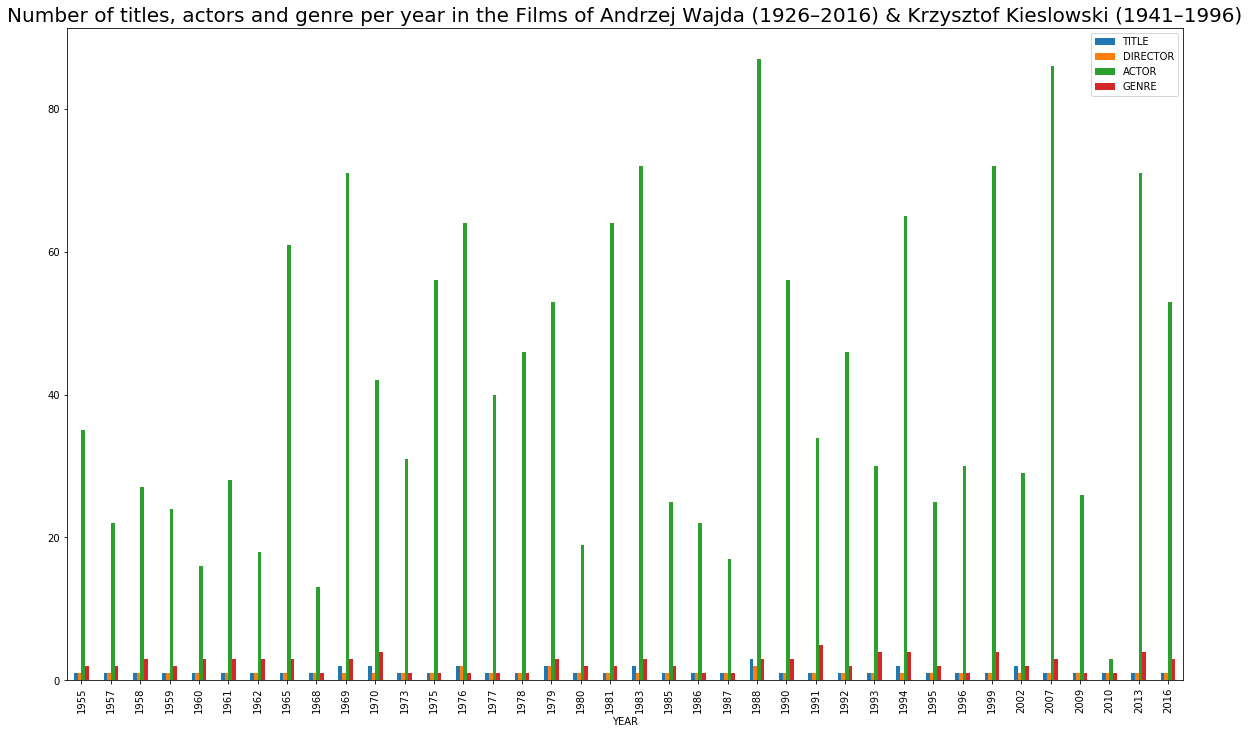
\includegraphics[width=11cm]{Figs/1_bars.png} \hspace*{6cm}
\end{center}

\end{frame}







\begin{frame}
\frametitle{The Graph of Aggregated Exchanges in Political Affiliation}
%\frametitle{The Graph of Aggregated Committees in Political Affiliation}

\begin{center}
\includegraphics[width=11.5cm]{Figs/3_1_GraphOfAggregatedCommittees1.png} \hspace*{4cm}
\end{center}

\end{frame}



\begin{frame}
\frametitle{The Heatmap of Aggregated Exchanges in Political Affiliation}
%\frametitle{The Adjacency Matrix of the Graph of Aggregated Committees in Political Affiliation}
\vspace{-0.3cm}
\begin{center}
\includegraphics[width=8cm]{Figs/3_1_a.png} \hspace*{4cm}
\end{center}

\end{frame}




\begin{frame}
\frametitle{\small Average Centralities of Aggregated Committees in Political Affiliation}

\begin{center}
\includegraphics[width=11.4cm]{Figs/avcen.png} \hspace*{4cm}
\end{center}

\end{frame}



\begin{frame}
\frametitle{Counts of Labeled Reciprocating Dyads}

\begin{table}[!htb]
\centering
\begin{tabular}{lr}
\toprule
               {\bf{Labelled Dyad}} &       {\bf{Count}} \\
\midrule

Uncategorized $\leftrightarrow$ Uncategorized & 23,652\\
REP $\leftrightarrow$  Uncategorized & 6,690\\
DEM  $\leftrightarrow$  Uncategorized & 5,200\\
DEM $\leftrightarrow$ DEM & 1,229\\
REP $\leftrightarrow$  REP & 815\\
Left Lean $\leftrightarrow$ Uncategorized & 44\\
Alternate $\leftrightarrow$ Alternate & 9\\
DEM  $\leftrightarrow$ Left Lean & 8\\
Alternate $\leftrightarrow$ Uncategorized & 6\\
REP $\leftrightarrow$  Right Lean & 3\\
Left Lean $\leftrightarrow$ Left Lean & 2\\
\bottomrule
\end{tabular}
\end{table}

\end{frame}





\begin{frame}
\frametitle{Graphs of Labelled Reciprocating Dyads}

\begin{center}
\Large
\begin{itemize}
\item DEM $\leftrightarrow$ DEM%| $=$ 1,229
\item REP $\leftrightarrow$ REP%| $=$  815
\item $\{$DEM, REP, Left Lean, Right Lean$\}$ $\leftrightarrow$ \\ $\{$DEM, REP, Left Lean, Right Lean$\}$%| $=$ 17
\end{itemize}
\end{center}

\end{frame}


\begin{frame}
\frametitle{DEM $\leftrightarrow$ DEM \phantom{This text will be invisible be invisible} \href{http://politicalnets.com/view/gcc_ddr}{\texttt{\textcolor{white}{Link}}}} 

\begin{center}
\includegraphics[width=9cm]{Figs/3_3_TheGraphofDEMReciprocators.png} \hspace*{4cm}
\end{center}

\end{frame}


\begin{frame}
\frametitle{REP $\leftrightarrow$ REP \phantom{This text will be invisible be invisible} \href{http://politicalnets.com/view/gcc_rrr}{\texttt{\textcolor{white}{Link}}}}

\begin{center}
\includegraphics[width=9.5cm]{Figs/3_2_TheGraphofREPReciprocators.png} \hspace*{4cm}
\end{center}

\end{frame}



\begin{frame}
\frametitle{\scriptsize $\{$DEM, REP, Left Lean, Right Lean$\}$ $\leftrightarrow$ $\{$DEM, REP, Left Lean, Right Lean$\}$  \phantom{This text} \href{http://politicalnets.com/view/otherr}{\texttt{\textcolor{white}{Link}}}}

\begin{center}
\includegraphics[width=10cm]{Figs/3_4_TheGraphofReciprocatorsamongDEM,REP,LeftLeanandRightLean.png} \hspace*{4cm}
\end{center}

\end{frame}




\begin{frame}
\frametitle{Counts of Labelled Co--Giving Triads}
\vspace{-0.3cm}
\small

\begin{table}[!htb]
\centering
Top 5 Labelled Co--Giving Triads
\begin{tabular}{lrr}
\toprule
               {\bf{Labelled Co--Giving Triad}} &       {\bf{Count}} & {\bf{Unique Givers}} \\
\midrule

DEM $\leftarrow$ Uncategorized $\rightarrow$ REP & 3,744,544 & 2,424\\
DEM $\leftarrow$ Uncategorized $\rightarrow$ DEM & 3,368,273 & 3,155\\
DEM  $\leftarrow$  Uncategorized $\rightarrow$ Uncategorized & 2,941,656 & 2,712\\
REP  $\leftarrow$  Uncategorized $\rightarrow$ REP & 2,786,801 & 3,117\\
REP  $\leftarrow$  Uncategorized $\rightarrow$ Uncategorized & 2,742,683 & 2,771\\
\bottomrule
\end{tabular}
\end{table}

\begin{table}[!htb]
\centering
Bottom 5 Labelled Co--Giving Triads
\begin{tabular}{lrr}
\toprule
               {\bf{Labelled Co--Giving Triad}} &       {\bf{Count}} & {\bf{Unique Givers}} \\
\midrule

Left Lean  $\leftarrow$  Uncategorized $\rightarrow$ Alternate & 7 & 5\\
Alternate  $\leftarrow$  Uncategorized $\rightarrow$ Alternate & 6 & 2\\
DEM $\leftarrow$ REP $\rightarrow$ Alternate & 5 & 3\\
Left Lean  $\leftarrow$  Left Lean $\rightarrow$ Left Lean & 5 & 3\\
DEM  $\leftarrow$  Uncategorized $\rightarrow$ Right Lean & 5 & 1\\
\bottomrule
\end{tabular}
\end{table}

\end{frame}





\begin{frame}
\frametitle{Graphs of Labelled Co-Giving Triads}

\begin{center}
\Large
\begin{itemize}
\item DEM $\leftarrow$ REP $\rightarrow$ DEM %| $=$ 847
\item REP $\leftarrow$ DEM $\rightarrow$ REP%| $=$ 1,443
\item $\{$DEM, REP$\}$ $\leftarrow$ $\{$Left Lean, Right Lean,Alternate$\}$ $\rightarrow$ $\{$DEM, REP$\}$%| $=$ 
\end{itemize}
\end{center}

\end{frame}


\begin{frame}
\frametitle{DEM $\leftarrow$ REP $\rightarrow$ DEM  \phantom{This text will be invisibleeee} \href{http://politicalnets.com/view/ddrr}{\texttt{\textcolor{white}{Link}}}}

\begin{center}
\includegraphics[width=9cm]{Figs/3_9_TheGraphofDEM-DEMReceivingbyREP.png} \hspace*{4cm}
\end{center}

\end{frame}


\begin{frame}
\frametitle{REP $\leftarrow$ DEM $\rightarrow$ REP  \phantom{This text will be invi} \href{http://politicalnets.com/view/rrrd}{\texttt{\textcolor{white}{Link}}}}
%$\rightarrow$ DEM  

\begin{center}
\includegraphics[width=9.5cm]{Figs/3_8_TheGraphofREP-REPReceivingbyDEM.png} \hspace*{4cm}
\end{center}

\end{frame}



\begin{frame}
\frametitle{\small $\{$DEM, REP$\}$ $\leftarrow$ $\{$Left Lean, Right Lean,Alternate$\}$ $\rightarrow$ $\{$DEM, REP$\}$   $\rightarrow$ DEM  \phantom{This text will be invisibleeeeThis text will be invisibleeeenvisibleeeeeeeee} \href{http://politicalnets.com/view/rother}{\texttt{\textcolor{white}{Link}}}}

\begin{center}
\includegraphics[width=9.5cm]{Figs/3_10_Left,RightLeanandAlternateReceivingbyDEMandREP.png} \hspace*{4cm}
\end{center}

\end{frame}






\begin{frame}
\frametitle{Counts of Labelled Co--Receiving Triads}
\vspace{-0.3cm}
\scriptsize

\begin{table}[!htb]
\centering
Top 5 Labelled Co--Giving Triads
\begin{tabular}{lrr}
\toprule
               {\bf{Labelled Co--Receiving Triad}} &       {\bf{Count}} & {\bf{Unique Receivers}} \\
\midrule

Uncategorized $\rightarrow$ REP  $\leftarrow$ Uncategorized & 11,517,614 & 798\\
Uncategorized $\rightarrow$ DEM  $\leftarrow$ Uncategorized & 9,760,559 & 744\\
Uncategorized $\rightarrow$ Uncategorized  $\leftarrow$ Uncategorized & 2,121,018 & 2963\\
DEM $\rightarrow$ DEM  $\leftarrow$ Uncategorized & 1,664,159 & 709\\
REP $\rightarrow$ REP  $\leftarrow$ Uncategorized & 1,453,265 & 731\\
\bottomrule
\end{tabular}
\end{table}

\begin{table}[!htb]
\centering
Bottom 5 Labelled Co--Giving Triads
\begin{tabular}{lrr}
\toprule
               {\bf{Labelled Co--Receiving Triad}} &       {\bf{Count}} & {\bf{Unique Receivers}} \\
\midrule

REP  $\rightarrow$  Alternate $\leftarrow$ REP & 7 & 2\\
REP  $\rightarrow$  Uncategorized $\leftarrow$ Alternate & 7 & 2\\
REP  $\rightarrow$  DEM $\leftarrow$ Left Lean & 4 & 4\\
Left Lean $\rightarrow$ Left Lean $\leftarrow$ Left Lean & 3 & 1\\
REP  $\rightarrow$  Left Lean $\leftarrow$ Left Lean & 1 & 1\\
\bottomrule
\end{tabular}
\end{table}

\end{frame}




\begin{frame}
\frametitle{Graphs of Labelled Co--Receiving Triads}

\begin{center}
\Large
\begin{itemize}
\item DEM $\rightarrow$ REP $\leftarrow$ DEM
\item REP $\rightarrow$ DEM $\leftarrow$ REP
\item $\{$DEM, REP,Left Lean$\}$ $\rightarrow$ $\{$Left Lean, Right Lean$\}$ $\leftarrow$ $\{$DEM, REP,Left Lean$\}$
\end{itemize}
\end{center}

\end{frame}


\begin{frame}
\frametitle{DEM $\rightarrow$ REP $\leftarrow$ DEM   \phantom{This text will be invisibleeee} \href{http://politicalnets.com/view/ddgr}{\texttt{\textcolor{white}{Link}}}}

\begin{center}
\includegraphics[width=9cm]{Figs/3_6_TheGraphofDEM-DEMGivingtoREP.png} \hspace*{4cm}
\end{center}

\end{frame}


\begin{frame}
\frametitle{REP $\rightarrow$ DEM $\leftarrow$ REP   \phantom{This text will be invisibleeee} \href{http://politicalnets.com/view/rrgd}{\texttt{\textcolor{white}{Link}}}}

\begin{center}
\includegraphics[width=9.5cm]{Figs/3_5_TheGraphofREP-REPGivingtoDEM.png} \hspace*{4cm}
\end{center}

\end{frame}



\begin{frame}
\frametitle{\small $\{$DEM, REP,Left Lean$\}$ $\rightarrow$ $\{$Left Lean, Right Lean$\}$ $\leftarrow$ $\{$DEM, REP,Left Lean$\}$ \phantom{This text will be invisibleeeeThis text will be invisibleeeenvisibleeeeeeeee} \href{http://politicalnets.com/view/drga}{\texttt{\textcolor{white}{Link}}}}

\begin{center}
\includegraphics[width=9cm]{Figs/3_7_DEMandREPGivingtoLeftandRightLean.png} \hspace*{4cm}
\end{center}

\end{frame}









\begin{frame}[plain,c,label=L4]

\begin{center}
\Huge {\bf{\color{brown}Conclusions}}
\end{center}

\end{frame}






\begin{frame}
\frametitle{Conclusions}

\begin{itemize}
\item Within party financial exchanges dominate the overall FEC network.
\item However,  we observed a number of some significant across--party financial exchanges,  despite some of the parties being in political opposition to each other.
\item The committees that are uncategorized (or unaffiliated) have the largest share among those exchanges that are not within a single party.
\item In upcoming and future elections it will be interesting to explore whether patterns observed here continue to hold.
\item We plan to further develop this data \& network analysis,  particularly expanded statistical analyses,  and welcome possible collaboration from the audience here among those interested.
\end{itemize}

\end{frame}























\end{document}